\documentclass[1p]{elsarticle_modified}
%\bibliographystyle{elsarticle-num}

%\usepackage[colorlinks]{hyperref}
%\usepackage{abbrmath_seonhwa} %\Abb, \Ascr, \Acal ,\Abf, \Afrak
\usepackage{amsfonts}
\usepackage{amssymb}
\usepackage{amsmath}
\usepackage{amsthm}
\usepackage{scalefnt}
\usepackage{amsbsy}
\usepackage{kotex}
\usepackage{caption}
\usepackage{subfig}
\usepackage{color}
\usepackage{graphicx}
\usepackage{xcolor} %% white, black, red, green, blue, cyan, magenta, yellow
\usepackage{float}
\usepackage{setspace}
\usepackage{hyperref}

\usepackage{tikz}
\usetikzlibrary{arrows}

\usepackage{multirow}
\usepackage{array} % fixed length table
\usepackage{hhline}

%%%%%%%%%%%%%%%%%%%%%
\makeatletter
\renewcommand*\env@matrix[1][\arraystretch]{%
	\edef\arraystretch{#1}%
	\hskip -\arraycolsep
	\let\@ifnextchar\new@ifnextchar
	\array{*\c@MaxMatrixCols c}}
\makeatother %https://tex.stackexchange.com/questions/14071/how-can-i-increase-the-line-spacing-in-a-matrix
%%%%%%%%%%%%%%%

\usepackage[normalem]{ulem}

\newcommand{\msout}[1]{\ifmmode\text{\sout{\ensuremath{#1}}}\else\sout{#1}\fi}
%SOURCE: \msout is \stkout macro in https://tex.stackexchange.com/questions/20609/strikeout-in-math-mode

\newcommand{\cancel}[1]{
	\ifmmode
	{\color{red}\msout{#1}}
	\else
	{\color{red}\sout{#1}}
	\fi
}

\newcommand{\add}[1]{
	{\color{blue}\uwave{#1}}
}

\newcommand{\replace}[2]{
	\ifmmode
	{\color{red}\msout{#1}}{\color{blue}\uwave{#2}}
	\else
	{\color{red}\sout{#1}}{\color{blue}\uwave{#2}}
	\fi
}

\newcommand{\Sol}{\mathcal{S}} %segment
\newcommand{\D}{D} %diagram
\newcommand{\A}{\mathcal{A}} %arc


%%%%%%%%%%%%%%%%%%%%%%%%%%%%%5 test

\def\sl{\operatorname{\textup{SL}}(2,\Cbb)}
\def\psl{\operatorname{\textup{PSL}}(2,\Cbb)}
\def\quan{\mkern 1mu \triangleright \mkern 1mu}

\theoremstyle{definition}
\newtheorem{thm}{Theorem}[section]
\newtheorem{prop}[thm]{Proposition}
\newtheorem{lem}[thm]{Lemma}
\newtheorem{ques}[thm]{Question}
\newtheorem{cor}[thm]{Corollary}
\newtheorem{defn}[thm]{Definition}
\newtheorem{exam}[thm]{Example}
\newtheorem{rmk}[thm]{Remark}
\newtheorem{alg}[thm]{Algorithm}

\newcommand{\I}{\sqrt{-1}}
\begin{document}

%\begin{frontmatter}
%
%\title{Boundary parabolic representations of knots up to 8 crossings}
%
%%% Group authors per affiliation:
%\author{Yunhi Cho} 
%\address{Department of Mathematics, University of Seoul, Seoul, Korea}
%\ead{yhcho@uos.ac.kr}
%
%
%\author{Seonhwa Kim} %\fnref{s_kim}}
%\address{Center for Geometry and Physics, Institute for Basic Science, Pohang, 37673, Korea}
%\ead{ryeona17@ibs.re.kr}
%
%\author{Hyuk Kim}
%\address{Department of Mathematical Sciences, Seoul National University, Seoul 08826, Korea}
%\ead{hyukkim@snu.ac.kr}
%
%\author{Seokbeom Yoon}
%\address{Department of Mathematical Sciences, Seoul National University, Seoul, 08826,  Korea}
%\ead{sbyoon15@snu.ac.kr}
%
%\begin{abstract}
%We find all boundary parabolic representation of knots up to 8 crossings.
%
%\end{abstract}
%\begin{keyword}
%    \MSC[2010] 57M25 
%\end{keyword}
%
%\end{frontmatter}

%\linenumbers
%\tableofcontents
%
\newcommand\colored[1]{\textcolor{white}{\rule[-0.35ex]{0.8em}{1.4ex}}\kern-0.8em\color{red} #1}%
%\newcommand\colored[1]{\textcolor{white}{ #1}\kern-2.17ex	\textcolor{white}{ #1}\kern-1.81ex	\textcolor{white}{ #1}\kern-2.15ex\color{red}#1	}

{\Large $\underline{12a_{0019}~(K12a_{0019})}$}

\setlength{\tabcolsep}{10pt}
\renewcommand{\arraystretch}{1.6}
\vspace{1cm}\begin{tabular}{m{100pt}>{\centering\arraybackslash}m{274pt}}
\multirow{5}{120pt}{
	\centering
	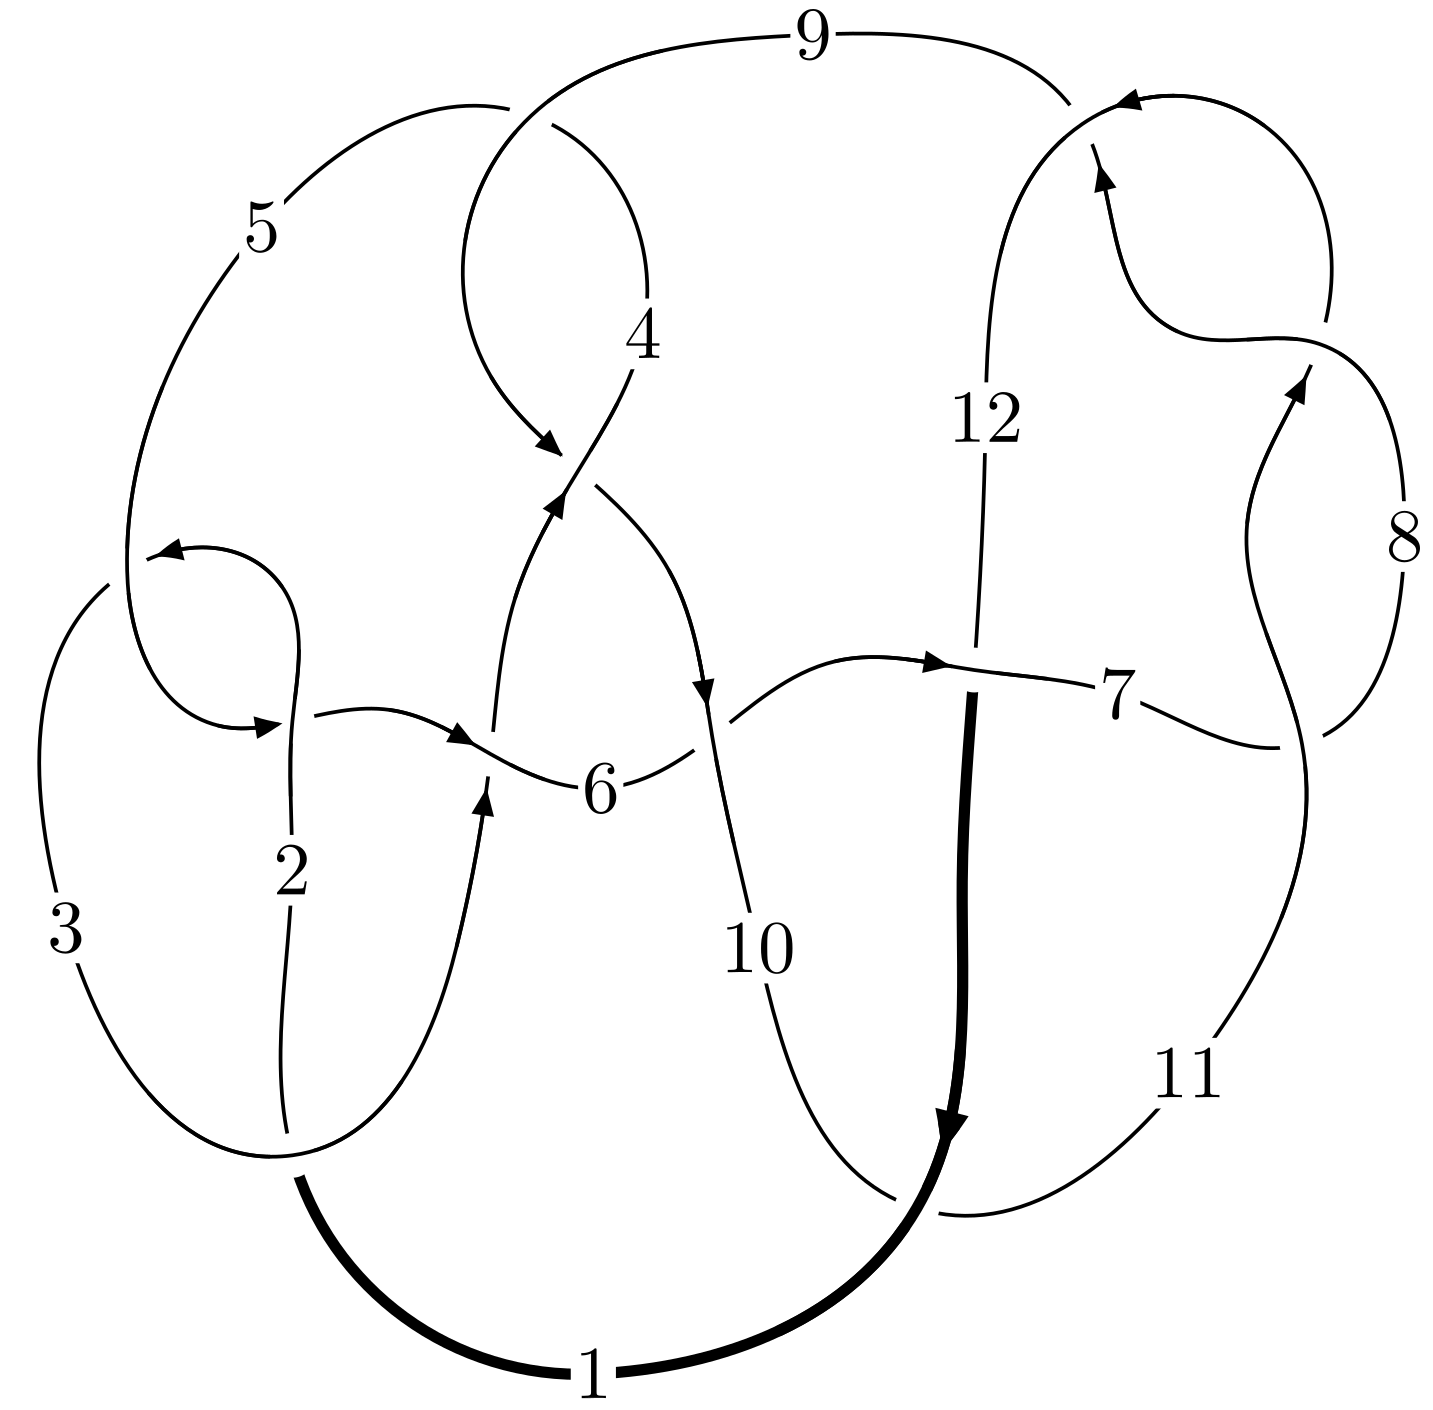
\includegraphics[width=112pt]{../../../GIT/diagram.site/Diagrams/png/820_12a_0019.png}\\
\ \ \ A knot diagram\footnotemark}&
\allowdisplaybreaks
\textbf{Linearized knot diagam} \\
\cline{2-2}
 &
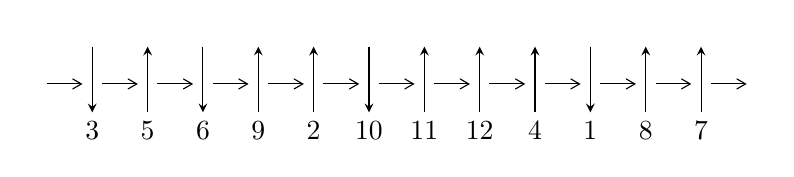
\begin{tikzpicture}[x=20pt, y=17pt]
	% nodes
	\node (C0) at (0, 0) {};
	\node (C1) at (1, 0) {};
	\node (C1U) at (1, +1) {};
	\node (C1D) at (1, -1) {3};

	\node (C2) at (2, 0) {};
	\node (C2U) at (2, +1) {};
	\node (C2D) at (2, -1) {5};

	\node (C3) at (3, 0) {};
	\node (C3U) at (3, +1) {};
	\node (C3D) at (3, -1) {6};

	\node (C4) at (4, 0) {};
	\node (C4U) at (4, +1) {};
	\node (C4D) at (4, -1) {9};

	\node (C5) at (5, 0) {};
	\node (C5U) at (5, +1) {};
	\node (C5D) at (5, -1) {2};

	\node (C6) at (6, 0) {};
	\node (C6U) at (6, +1) {};
	\node (C6D) at (6, -1) {10};

	\node (C7) at (7, 0) {};
	\node (C7U) at (7, +1) {};
	\node (C7D) at (7, -1) {11};

	\node (C8) at (8, 0) {};
	\node (C8U) at (8, +1) {};
	\node (C8D) at (8, -1) {12};

	\node (C9) at (9, 0) {};
	\node (C9U) at (9, +1) {};
	\node (C9D) at (9, -1) {4};

	\node (C10) at (10, 0) {};
	\node (C10U) at (10, +1) {};
	\node (C10D) at (10, -1) {1};

	\node (C11) at (11, 0) {};
	\node (C11U) at (11, +1) {};
	\node (C11D) at (11, -1) {8};

	\node (C12) at (12, 0) {};
	\node (C12U) at (12, +1) {};
	\node (C12D) at (12, -1) {7};
	\node (C13) at (13, 0) {};

	% arrows
	\draw[->,>={angle 60}]
	(C0) edge (C1) (C1) edge (C2) (C2) edge (C3) (C3) edge (C4) (C4) edge (C5) (C5) edge (C6) (C6) edge (C7) (C7) edge (C8) (C8) edge (C9) (C9) edge (C10) (C10) edge (C11) (C11) edge (C12) (C12) edge (C13) ;	\draw[->,>=stealth]
	(C1U) edge (C1D) (C2D) edge (C2U) (C3U) edge (C3D) (C4D) edge (C4U) (C5D) edge (C5U) (C6U) edge (C6D) (C7D) edge (C7U) (C8D) edge (C8U) (C9D) edge (C9U) (C10U) edge (C10D) (C11D) edge (C11U) (C12D) edge (C12U) ;
	\end{tikzpicture} \\
\hhline{~~} \\& 
\textbf{Solving Sequence} \\ \cline{2-2} 
 &
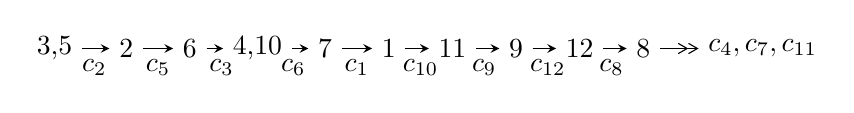
\begin{tikzpicture}[x=23pt, y=7pt]
	% node
	\node (A0) at (-1/8, 0) {3,5};
	\node (A1) at (1, 0) {2};
	\node (A2) at (2, 0) {6};
	\node (A3) at (49/16, 0) {4,10};
	\node (A4) at (33/8, 0) {7};
	\node (A5) at (41/8, 0) {1};
	\node (A6) at (49/8, 0) {11};
	\node (A7) at (57/8, 0) {9};
	\node (A8) at (65/8, 0) {12};
	\node (A9) at (73/8, 0) {8};
	\node (C1) at (1/2, -1) {$c_{2}$};
	\node (C2) at (3/2, -1) {$c_{5}$};
	\node (C3) at (5/2, -1) {$c_{3}$};
	\node (C4) at (29/8, -1) {$c_{6}$};
	\node (C5) at (37/8, -1) {$c_{1}$};
	\node (C6) at (45/8, -1) {$c_{10}$};
	\node (C7) at (53/8, -1) {$c_{9}$};
	\node (C8) at (61/8, -1) {$c_{12}$};
	\node (C9) at (69/8, -1) {$c_{8}$};
	\node (A10) at (11, 0) {$c_{4},c_{7},c_{11}$};

	% edge
	\draw[->,>=stealth]	
	(A0) edge (A1) (A1) edge (A2) (A2) edge (A3) (A3) edge (A4) (A4) edge (A5) (A5) edge (A6) (A6) edge (A7) (A7) edge (A8) (A8) edge (A9) ;
	\draw[->>,>={angle 60}]	
	(A9) edge (A10);
\end{tikzpicture} \\ 

\end{tabular} \\

\footnotetext{
The image of knot diagram is generated by the software ``\textbf{Draw programme}" developed by Andrew Bartholomew(\url{http://www.layer8.co.uk/maths/draw/index.htm\#Running-draw}), where we modified some parts for our purpose(\url{https://github.com/CATsTAILs/LinksPainter}).
}\phantom \\ \newline 
\centering \textbf{Ideals for irreducible components\footnotemark of $X_{\text{par}}$} 
 
\begin{align*}
I^u_{1}&=\langle 
205 u^{104}-998 u^{103}+\cdots+16 b-31,\;2 u^{104}-29 u^{103}+\cdots+8 a+71,\;u^{105}-6 u^{104}+\cdots-5 u+1\rangle \\
I^u_{2}&=\langle 
b^5- b^4 u- b^4+2 b^3 u+b^2- b u- b+u,\;a,\;u^2+u+1\rangle \\
\\
\end{align*}
\raggedright * 2 irreducible components of $\dim_{\mathbb{C}}=0$, with total 115 representations.\\
\footnotetext{All coefficients of polynomials are rational numbers. But the coefficients are sometimes approximated in decimal forms when there is not enough margin.}
\newpage
\renewcommand{\arraystretch}{1}
\centering \section*{I. $I^u_{1}= \langle 205 u^{104}-998 u^{103}+\cdots+16 b-31,\;2 u^{104}-29 u^{103}+\cdots+8 a+71,\;u^{105}-6 u^{104}+\cdots-5 u+1 \rangle$}
\flushleft \textbf{(i) Arc colorings}\\
\begin{tabular}{m{7pt} m{180pt} m{7pt} m{180pt} }
\flushright $a_{3}=$&$\begin{pmatrix}1\\0\end{pmatrix}$ \\
\flushright $a_{5}=$&$\begin{pmatrix}0\\u\end{pmatrix}$ \\
\flushright $a_{2}=$&$\begin{pmatrix}1\\u^2\end{pmatrix}$ \\
\flushright $a_{6}=$&$\begin{pmatrix}u\\u^3+u\end{pmatrix}$ \\
\flushright $a_{4}=$&$\begin{pmatrix}u^4+u^2+1\\u^6+2 u^4+u^2\end{pmatrix}$ \\
\flushright $a_{10}=$&$\begin{pmatrix}-0.250000 u^{104}+3.62500 u^{103}+\cdots+23.2500 u-8.87500\\-12.8125 u^{104}+62.3750 u^{103}+\cdots-10.4375 u+1.93750\end{pmatrix}$ \\
\flushright $a_{7}=$&$\begin{pmatrix}u^{12}+3 u^{10}+5 u^8-2 u^7+4 u^6-4 u^5+2 u^4-4 u^3+u^2+1\\-0.0625000 u^{103}+0.312500 u^{102}+\cdots+0.250000 u-0.0625000\end{pmatrix}$ \\
\flushright $a_{1}=$&$\begin{pmatrix}u^2+1\\u^2\end{pmatrix}$ \\
\flushright $a_{11}=$&$\begin{pmatrix}-19.3125 u^{104}+82.4375 u^{103}+\cdots+46.6875 u-19.2500\\-\frac{97}{2} u^{104}+\frac{1993}{8} u^{103}+\cdots-68 u+\frac{81}{8}\end{pmatrix}$ \\
\flushright $a_{9}=$&$\begin{pmatrix}-15.2500 u^{104}+69.6250 u^{103}+\cdots+24.2500 u-11.8750\\-37.9375 u^{104}+192.875 u^{103}+\cdots-43.8125 u+6.81250\end{pmatrix}$ \\
\flushright $a_{12}=$&$\begin{pmatrix}-0.187500 u^{104}+1.12500 u^{103}+\cdots-0.937500 u+1.18750\\-1.43750 u^{104}+6.93750 u^{103}+\cdots+0.0625000 u-0.375000\end{pmatrix}$ \\
\flushright $a_{8}=$&$\begin{pmatrix}-0.250000 u^{104}+2.68750 u^{103}+\cdots-6.12500 u+1.43750\\2.62500 u^{104}-12.5625 u^{103}+\cdots+0.375000 u+0.812500\end{pmatrix}$\\&\end{tabular}
\flushleft \textbf{(ii) Obstruction class $= -1$}\\~\\
\flushleft \textbf{(iii) Cusp Shapes $= -\frac{461}{16} u^{104}+\frac{3579}{16} u^{103}+\cdots-\frac{4979}{16} u+\frac{163}{2}$}\\~\\
\newpage\renewcommand{\arraystretch}{1}
\flushleft \textbf{(iv) u-Polynomials at the component}\newline \\
\begin{tabular}{m{50pt}|m{274pt}}
Crossings & \hspace{64pt}u-Polynomials at each crossing \\
\hline $$\begin{aligned}c_{1}\end{aligned}$$&$\begin{aligned}
&u^{105}+52 u^{104}+\cdots-5 u-1
\end{aligned}$\\
\hline $$\begin{aligned}c_{2},c_{5}\end{aligned}$$&$\begin{aligned}
&u^{105}+6 u^{104}+\cdots-5 u-1
\end{aligned}$\\
\hline $$\begin{aligned}c_{3}\end{aligned}$$&$\begin{aligned}
&u^{105}-6 u^{104}+\cdots+107353 u-23497
\end{aligned}$\\
\hline $$\begin{aligned}c_{4},c_{9}\end{aligned}$$&$\begin{aligned}
&u^{105}+u^{104}+\cdots+1024 u-1024
\end{aligned}$\\
\hline $$\begin{aligned}c_{6}\end{aligned}$$&$\begin{aligned}
&u^{105}+3 u^{104}+\cdots-1465582 u-149381
\end{aligned}$\\
\hline $$\begin{aligned}c_{7},c_{8},c_{11}\end{aligned}$$&$\begin{aligned}
&u^{105}-3 u^{104}+\cdots-2 u-1
\end{aligned}$\\
\hline $$\begin{aligned}c_{10}\end{aligned}$$&$\begin{aligned}
&u^{105}-23 u^{104}+\cdots+167398 u-8023
\end{aligned}$\\
\hline $$\begin{aligned}c_{12}\end{aligned}$$&$\begin{aligned}
&u^{105}+9 u^{104}+\cdots+6 u+1
\end{aligned}$\\
\hline
\end{tabular}\\~\\
\newpage\renewcommand{\arraystretch}{1}
\flushleft \textbf{(v) Riley Polynomials at the component}\newline \\
\begin{tabular}{m{50pt}|m{274pt}}
Crossings & \hspace{64pt}Riley Polynomials at each crossing \\
\hline $$\begin{aligned}c_{1}\end{aligned}$$&$\begin{aligned}
&y^{105}+8 y^{104}+\cdots-21 y-1
\end{aligned}$\\
\hline $$\begin{aligned}c_{2},c_{5}\end{aligned}$$&$\begin{aligned}
&y^{105}+52 y^{104}+\cdots-5 y-1
\end{aligned}$\\
\hline $$\begin{aligned}c_{3}\end{aligned}$$&$\begin{aligned}
&y^{105}-36 y^{104}+\cdots+985651187 y-552109009
\end{aligned}$\\
\hline $$\begin{aligned}c_{4},c_{9}\end{aligned}$$&$\begin{aligned}
&y^{105}+55 y^{104}+\cdots-25165824 y-1048576
\end{aligned}$\\
\hline $$\begin{aligned}c_{6}\end{aligned}$$&$\begin{aligned}
&y^{105}-31 y^{104}+\cdots+449047075542 y-22314683161
\end{aligned}$\\
\hline $$\begin{aligned}c_{7},c_{8},c_{11}\end{aligned}$$&$\begin{aligned}
&y^{105}-95 y^{104}+\cdots+2 y-1
\end{aligned}$\\
\hline $$\begin{aligned}c_{10}\end{aligned}$$&$\begin{aligned}
&y^{105}+29 y^{104}+\cdots-2885666658 y-64368529
\end{aligned}$\\
\hline $$\begin{aligned}c_{12}\end{aligned}$$&$\begin{aligned}
&y^{105}-3 y^{104}+\cdots+14 y-1
\end{aligned}$\\
\hline
\end{tabular}\\~\\
\newpage\flushleft \textbf{(vi) Complex Volumes and Cusp Shapes}
$$\begin{array}{c|c|c}  
\text{Solutions to }I^u_{1}& \I (\text{vol} + \sqrt{-1}CS) & \text{Cusp shape}\\
 \hline 
\begin{aligned}
u &= -0.238259 + 0.986456 I \\
a &= -1.26147 - 0.77818 I \\
b &= -0.958466 + 0.563608 I\end{aligned}
 & \phantom{-}3.17345 - 4.25894 I & \phantom{-0.000000 } 0 \\ \hline\begin{aligned}
u &= -0.238259 - 0.986456 I \\
a &= -1.26147 + 0.77818 I \\
b &= -0.958466 - 0.563608 I\end{aligned}
 & \phantom{-}3.17345 + 4.25894 I & \phantom{-0.000000 } 0 \\ \hline\begin{aligned}
u &= -0.713466 + 0.725019 I \\
a &= -0.078403 - 0.675734 I \\
b &= -0.507694 + 0.558076 I\end{aligned}
 & -0.27464 - 5.50436 I & \phantom{-0.000000 } 0 \\ \hline\begin{aligned}
u &= -0.713466 - 0.725019 I \\
a &= -0.078403 + 0.675734 I \\
b &= -0.507694 - 0.558076 I\end{aligned}
 & -0.27464 + 5.50436 I & \phantom{-0.000000 } 0 \\ \hline\begin{aligned}
u &= -0.736153 + 0.712752 I \\
a &= \phantom{-}0.194353 + 0.806457 I \\
b &= \phantom{-}0.794010 - 0.666918 I\end{aligned}
 & \phantom{-}5.05878 - 8.91753 I & \phantom{-0.000000 } 0 \\ \hline\begin{aligned}
u &= -0.736153 - 0.712752 I \\
a &= \phantom{-}0.194353 - 0.806457 I \\
b &= \phantom{-}0.794010 + 0.666918 I\end{aligned}
 & \phantom{-}5.05878 + 8.91753 I & \phantom{-0.000000 } 0 \\ \hline\begin{aligned}
u &= -0.671892 + 0.802497 I \\
a &= -0.092701 + 0.249210 I \\
b &= -0.325633 - 0.405265 I\end{aligned}
 & \phantom{-}1.28850 - 2.57717 I & \phantom{-0.000000 } 0 \\ \hline\begin{aligned}
u &= -0.671892 - 0.802497 I \\
a &= -0.092701 - 0.249210 I \\
b &= -0.325633 + 0.405265 I\end{aligned}
 & \phantom{-}1.28850 + 2.57717 I & \phantom{-0.000000 } 0 \\ \hline\begin{aligned}
u &= -0.638895 + 0.706476 I \\
a &= -0.318007 + 0.601750 I \\
b &= \phantom{-}0.235155 + 0.010258 I\end{aligned}
 & \phantom{-}1.04013 - 2.17525 I & \phantom{-0.000000 } 0 \\ \hline\begin{aligned}
u &= -0.638895 - 0.706476 I \\
a &= -0.318007 - 0.601750 I \\
b &= \phantom{-}0.235155 - 0.010258 I\end{aligned}
 & \phantom{-}1.04013 + 2.17525 I & \phantom{-0.000000 } 0\\
 \hline 
 \end{array}$$\newpage$$\begin{array}{c|c|c}  
\text{Solutions to }I^u_{1}& \I (\text{vol} + \sqrt{-1}CS) & \text{Cusp shape}\\
 \hline 
\begin{aligned}
u &= -0.689517 + 0.630908 I \\
a &= \phantom{-}0.364134 - 1.084130 I \\
b &= -0.817093 - 0.314730 I\end{aligned}
 & \phantom{-}6.79137 - 0.46918 I & \phantom{-0.000000 } 0 \\ \hline\begin{aligned}
u &= -0.689517 - 0.630908 I \\
a &= \phantom{-}0.364134 + 1.084130 I \\
b &= -0.817093 + 0.314730 I\end{aligned}
 & \phantom{-}6.79137 + 0.46918 I & \phantom{-0.000000 } 0 \\ \hline\begin{aligned}
u &= -0.574800 + 0.919200 I \\
a &= -0.397771 + 0.333368 I \\
b &= -0.310416 + 0.660624 I\end{aligned}
 & \phantom{-}0.42904 - 2.56514 I & \phantom{-0.000000 } 0 \\ \hline\begin{aligned}
u &= -0.574800 - 0.919200 I \\
a &= -0.397771 - 0.333368 I \\
b &= -0.310416 - 0.660624 I\end{aligned}
 & \phantom{-}0.42904 + 2.56514 I & \phantom{-0.000000 } 0 \\ \hline\begin{aligned}
u &= \phantom{-}0.840312 + 0.309790 I \\
a &= -2.27824 - 0.15338 I \\
b &= -1.68105 - 1.17690 I\end{aligned}
 & \phantom{-}2.76203 - 11.75360 I & \phantom{-0.000000 } 0 \\ \hline\begin{aligned}
u &= \phantom{-}0.840312 - 0.309790 I \\
a &= -2.27824 + 0.15338 I \\
b &= -1.68105 + 1.17690 I\end{aligned}
 & \phantom{-}2.76203 + 11.75360 I & \phantom{-0.000000 } 0 \\ \hline\begin{aligned}
u &= -0.665816 + 0.883086 I \\
a &= \phantom{-}0.305710 + 0.000397 I \\
b &= \phantom{-}1.015970 - 0.021122 I\end{aligned}
 & -0.741803 + 0.253440 I & \phantom{-0.000000 } 0 \\ \hline\begin{aligned}
u &= -0.665816 - 0.883086 I \\
a &= \phantom{-}0.305710 - 0.000397 I \\
b &= \phantom{-}1.015970 + 0.021122 I\end{aligned}
 & -0.741803 - 0.253440 I & \phantom{-0.000000 } 0 \\ \hline\begin{aligned}
u &= \phantom{-}0.831615 + 0.295643 I \\
a &= \phantom{-}2.15583 + 0.06101 I \\
b &= \phantom{-}1.63171 + 0.91797 I\end{aligned}
 & -2.67355 - 8.10755 I & \phantom{-0.000000 } 0 \\ \hline\begin{aligned}
u &= \phantom{-}0.831615 - 0.295643 I \\
a &= \phantom{-}2.15583 - 0.06101 I \\
b &= \phantom{-}1.63171 - 0.91797 I\end{aligned}
 & -2.67355 + 8.10755 I & \phantom{-0.000000 } 0\\
 \hline 
 \end{array}$$\newpage$$\begin{array}{c|c|c}  
\text{Solutions to }I^u_{1}& \I (\text{vol} + \sqrt{-1}CS) & \text{Cusp shape}\\
 \hline 
\begin{aligned}
u &= \phantom{-}0.452334 + 1.030860 I \\
a &= -0.183842 - 0.270970 I \\
b &= -1.360810 - 0.270591 I\end{aligned}
 & \phantom{-}4.93430 - 1.63016 I & \phantom{-0.000000 } 0 \\ \hline\begin{aligned}
u &= \phantom{-}0.452334 - 1.030860 I \\
a &= -0.183842 + 0.270970 I \\
b &= -1.360810 + 0.270591 I\end{aligned}
 & \phantom{-}4.93430 + 1.63016 I & \phantom{-0.000000 } 0 \\ \hline\begin{aligned}
u &= -0.217271 + 0.841985 I \\
a &= \phantom{-}1.089980 + 0.405677 I \\
b &= \phantom{-}0.655102 - 0.510945 I\end{aligned}
 & -1.45249 - 1.72915 I & \phantom{-0.000000 } 0 \\ \hline\begin{aligned}
u &= -0.217271 - 0.841985 I \\
a &= \phantom{-}1.089980 - 0.405677 I \\
b &= \phantom{-}0.655102 + 0.510945 I\end{aligned}
 & -1.45249 + 1.72915 I & \phantom{-0.000000 } 0 \\ \hline\begin{aligned}
u &= -0.681527 + 0.905951 I \\
a &= -0.382548 - 0.129469 I \\
b &= -1.384110 + 0.114120 I\end{aligned}
 & \phantom{-}4.48814 + 3.55358 I & \phantom{-0.000000 } 0 \\ \hline\begin{aligned}
u &= -0.681527 - 0.905951 I \\
a &= -0.382548 + 0.129469 I \\
b &= -1.384110 - 0.114120 I\end{aligned}
 & \phantom{-}4.48814 - 3.55358 I & \phantom{-0.000000 } 0 \\ \hline\begin{aligned}
u &= -0.623618 + 0.962160 I \\
a &= \phantom{-}0.721379 - 0.227987 I \\
b &= \phantom{-}0.86546 - 1.18166 I\end{aligned}
 & \phantom{-}5.81874 - 4.58356 I & \phantom{-0.000000 } 0 \\ \hline\begin{aligned}
u &= -0.623618 - 0.962160 I \\
a &= \phantom{-}0.721379 + 0.227987 I \\
b &= \phantom{-}0.86546 + 1.18166 I\end{aligned}
 & \phantom{-}5.81874 + 4.58356 I & \phantom{-0.000000 } 0 \\ \hline\begin{aligned}
u &= \phantom{-}0.803505 + 0.279635 I \\
a &= -1.88136 - 0.03883 I \\
b &= -1.32765 - 0.58750 I\end{aligned}
 & -1.22209 - 4.21071 I & \phantom{-0.000000 } 0 \\ \hline\begin{aligned}
u &= \phantom{-}0.803505 - 0.279635 I \\
a &= -1.88136 + 0.03883 I \\
b &= -1.32765 + 0.58750 I\end{aligned}
 & -1.22209 + 4.21071 I & \phantom{-0.000000 } 0\\
 \hline 
 \end{array}$$\newpage$$\begin{array}{c|c|c}  
\text{Solutions to }I^u_{1}& \I (\text{vol} + \sqrt{-1}CS) & \text{Cusp shape}\\
 \hline 
\begin{aligned}
u &= \phantom{-}0.452689 + 1.056720 I \\
a &= \phantom{-}0.074853 + 0.313378 I \\
b &= \phantom{-}1.017450 + 0.224839 I\end{aligned}
 & -0.99128 + 1.45005 I & \phantom{-0.000000 } 0 \\ \hline\begin{aligned}
u &= \phantom{-}0.452689 - 1.056720 I \\
a &= \phantom{-}0.074853 - 0.313378 I \\
b &= \phantom{-}1.017450 - 0.224839 I\end{aligned}
 & -0.99128 - 1.45005 I & \phantom{-0.000000 } 0 \\ \hline\begin{aligned}
u &= \phantom{-}0.249719 + 1.127130 I \\
a &= -0.337353 + 0.825247 I \\
b &= -1.172070 + 0.570226 I\end{aligned}
 & \phantom{-}0.735634 + 0.034464 I & \phantom{-0.000000 } 0 \\ \hline\begin{aligned}
u &= \phantom{-}0.249719 - 1.127130 I \\
a &= -0.337353 - 0.825247 I \\
b &= -1.172070 - 0.570226 I\end{aligned}
 & \phantom{-}0.735634 - 0.034464 I & \phantom{-0.000000 } 0 \\ \hline\begin{aligned}
u &= -0.359634 + 1.100080 I \\
a &= \phantom{-}0.93545 + 1.83419 I \\
b &= \phantom{-}1.95166 - 0.28636 I\end{aligned}
 & \phantom{-}1.89142 + 2.96005 I & \phantom{-0.000000 } 0 \\ \hline\begin{aligned}
u &= -0.359634 - 1.100080 I \\
a &= \phantom{-}0.93545 - 1.83419 I \\
b &= \phantom{-}1.95166 + 0.28636 I\end{aligned}
 & \phantom{-}1.89142 - 2.96005 I & \phantom{-0.000000 } 0 \\ \hline\begin{aligned}
u &= -0.389409 + 1.089920 I \\
a &= -0.63466 - 1.82375 I \\
b &= -1.96185 - 0.06207 I\end{aligned}
 & -3.13580 - 0.41934 I & \phantom{-0.000000 } 0 \\ \hline\begin{aligned}
u &= -0.389409 - 1.089920 I \\
a &= -0.63466 + 1.82375 I \\
b &= -1.96185 + 0.06207 I\end{aligned}
 & -3.13580 + 0.41934 I & \phantom{-0.000000 } 0 \\ \hline\begin{aligned}
u &= \phantom{-}0.807528 + 0.227271 I \\
a &= -1.67463 + 0.33114 I \\
b &= -1.45547 + 0.03303 I\end{aligned}
 & -1.76859 - 4.38470 I & \phantom{-0.000000 } 0 \\ \hline\begin{aligned}
u &= \phantom{-}0.807528 - 0.227271 I \\
a &= -1.67463 - 0.33114 I \\
b &= -1.45547 - 0.03303 I\end{aligned}
 & -1.76859 + 4.38470 I & \phantom{-0.000000 } 0\\
 \hline 
 \end{array}$$\newpage$$\begin{array}{c|c|c}  
\text{Solutions to }I^u_{1}& \I (\text{vol} + \sqrt{-1}CS) & \text{Cusp shape}\\
 \hline 
\begin{aligned}
u &= \phantom{-}0.772794 + 0.325455 I \\
a &= \phantom{-}1.79242 + 0.44030 I \\
b &= \phantom{-}0.757606 + 0.919693 I\end{aligned}
 & \phantom{-}5.25845 - 2.77553 I & \phantom{-0.000000 } 0 \\ \hline\begin{aligned}
u &= \phantom{-}0.772794 - 0.325455 I \\
a &= \phantom{-}1.79242 - 0.44030 I \\
b &= \phantom{-}0.757606 - 0.919693 I\end{aligned}
 & \phantom{-}5.25845 + 2.77553 I & \phantom{-0.000000 } 0 \\ \hline\begin{aligned}
u &= \phantom{-}0.502800 + 1.057210 I \\
a &= \phantom{-}0.216151 + 0.559139 I \\
b &= \phantom{-}0.777715 + 0.999350 I\end{aligned}
 & \phantom{-}5.38886 + 8.04809 I & \phantom{-0.000000 } 0 \\ \hline\begin{aligned}
u &= \phantom{-}0.502800 - 1.057210 I \\
a &= \phantom{-}0.216151 - 0.559139 I \\
b &= \phantom{-}0.777715 - 0.999350 I\end{aligned}
 & \phantom{-}5.38886 - 8.04809 I & \phantom{-0.000000 } 0 \\ \hline\begin{aligned}
u &= \phantom{-}0.481039 + 1.072010 I \\
a &= -0.058829 - 0.497848 I \\
b &= -0.663625 - 0.543924 I\end{aligned}
 & -0.74038 + 5.32830 I & \phantom{-0.000000 } 0 \\ \hline\begin{aligned}
u &= \phantom{-}0.481039 - 1.072010 I \\
a &= -0.058829 + 0.497848 I \\
b &= -0.663625 + 0.543924 I\end{aligned}
 & -0.74038 - 5.32830 I & \phantom{-0.000000 } 0 \\ \hline\begin{aligned}
u &= -0.476095 + 1.075970 I \\
a &= -0.23047 + 1.70037 I \\
b &= \phantom{-}1.74561 + 1.18904 I\end{aligned}
 & -0.79779 - 3.44805 I & \phantom{-0.000000 } 0 \\ \hline\begin{aligned}
u &= -0.476095 - 1.075970 I \\
a &= -0.23047 - 1.70037 I \\
b &= \phantom{-}1.74561 - 1.18904 I\end{aligned}
 & -0.79779 + 3.44805 I & \phantom{-0.000000 } 0 \\ \hline\begin{aligned}
u &= -0.442891 + 1.094540 I \\
a &= \phantom{-}0.10056 + 1.92739 I \\
b &= \phantom{-}2.09472 + 0.74492 I\end{aligned}
 & -0.86758 - 3.63979 I & \phantom{-0.000000 } 0 \\ \hline\begin{aligned}
u &= -0.442891 - 1.094540 I \\
a &= \phantom{-}0.10056 - 1.92739 I \\
b &= \phantom{-}2.09472 - 0.74492 I\end{aligned}
 & -0.86758 + 3.63979 I & \phantom{-0.000000 } 0\\
 \hline 
 \end{array}$$\newpage$$\begin{array}{c|c|c}  
\text{Solutions to }I^u_{1}& \I (\text{vol} + \sqrt{-1}CS) & \text{Cusp shape}\\
 \hline 
\begin{aligned}
u &= -0.537994 + 1.060310 I \\
a &= \phantom{-}0.79040 - 1.33454 I \\
b &= -1.04542 - 1.96500 I\end{aligned}
 & \phantom{-}5.06634 - 2.14002 I & \phantom{-0.000000 } 0 \\ \hline\begin{aligned}
u &= -0.537994 - 1.060310 I \\
a &= \phantom{-}0.79040 + 1.33454 I \\
b &= -1.04542 + 1.96500 I\end{aligned}
 & \phantom{-}5.06634 + 2.14002 I & \phantom{-0.000000 } 0 \\ \hline\begin{aligned}
u &= \phantom{-}0.791185 + 0.177363 I \\
a &= \phantom{-}1.300070 - 0.513805 I \\
b &= \phantom{-}1.187640 - 0.524337 I\end{aligned}
 & -4.51741 - 0.87205 I & \phantom{-0.000000 } 0 \\ \hline\begin{aligned}
u &= \phantom{-}0.791185 - 0.177363 I \\
a &= \phantom{-}1.300070 + 0.513805 I \\
b &= \phantom{-}1.187640 + 0.524337 I\end{aligned}
 & -4.51741 + 0.87205 I & \phantom{-0.000000 } 0 \\ \hline\begin{aligned}
u &= \phantom{-}0.789318 + 0.130913 I \\
a &= -0.990302 + 0.696881 I \\
b &= -0.968136 + 0.899123 I\end{aligned}
 & \phantom{-}0.11479 + 2.61520 I & \phantom{-0.000000 } 0 \\ \hline\begin{aligned}
u &= \phantom{-}0.789318 - 0.130913 I \\
a &= -0.990302 - 0.696881 I \\
b &= -0.968136 - 0.899123 I\end{aligned}
 & \phantom{-}0.11479 - 2.61520 I & \phantom{-0.000000 } 0 \\ \hline\begin{aligned}
u &= -0.497296 + 1.109830 I \\
a &= \phantom{-}0.54471 - 2.03133 I \\
b &= -2.21310 - 1.70139 I\end{aligned}
 & -2.35810 - 6.97390 I & \phantom{-0.000000 } 0 \\ \hline\begin{aligned}
u &= -0.497296 - 1.109830 I \\
a &= \phantom{-}0.54471 + 2.03133 I \\
b &= -2.21310 + 1.70139 I\end{aligned}
 & -2.35810 + 6.97390 I & \phantom{-0.000000 } 0 \\ \hline\begin{aligned}
u &= \phantom{-}0.268185 + 1.187910 I \\
a &= -0.028682 - 1.225910 I \\
b &= \phantom{-}1.40267 - 0.59674 I\end{aligned}
 & -5.82532 - 0.95127 I & \phantom{-0.000000 } 0 \\ \hline\begin{aligned}
u &= \phantom{-}0.268185 - 1.187910 I \\
a &= -0.028682 + 1.225910 I \\
b &= \phantom{-}1.40267 + 0.59674 I\end{aligned}
 & -5.82532 + 0.95127 I & \phantom{-0.000000 } 0\\
 \hline 
 \end{array}$$\newpage$$\begin{array}{c|c|c}  
\text{Solutions to }I^u_{1}& \I (\text{vol} + \sqrt{-1}CS) & \text{Cusp shape}\\
 \hline 
\begin{aligned}
u &= \phantom{-}0.243554 + 1.203910 I \\
a &= -0.14026 + 1.48236 I \\
b &= -1.46102 + 0.43158 I\end{aligned}
 & -7.51174 - 4.84738 I & \phantom{-0.000000 } 0 \\ \hline\begin{aligned}
u &= \phantom{-}0.243554 - 1.203910 I \\
a &= -0.14026 - 1.48236 I \\
b &= -1.46102 - 0.43158 I\end{aligned}
 & -7.51174 + 4.84738 I & \phantom{-0.000000 } 0 \\ \hline\begin{aligned}
u &= -0.510942 + 1.117850 I \\
a &= -0.74030 + 2.08914 I \\
b &= \phantom{-}2.29397 + 2.01991 I\end{aligned}
 & \phantom{-}2.94950 - 10.49200 I & \phantom{-0.000000 } 0 \\ \hline\begin{aligned}
u &= -0.510942 - 1.117850 I \\
a &= -0.74030 - 2.08914 I \\
b &= \phantom{-}2.29397 - 2.01991 I\end{aligned}
 & \phantom{-}2.94950 + 10.49200 I & \phantom{-0.000000 } 0 \\ \hline\begin{aligned}
u &= \phantom{-}0.227624 + 1.207990 I \\
a &= \phantom{-}0.29337 - 1.57666 I \\
b &= \phantom{-}1.43638 - 0.32576 I\end{aligned}
 & -2.19295 - 8.54270 I & \phantom{-0.000000 } 0 \\ \hline\begin{aligned}
u &= \phantom{-}0.227624 - 1.207990 I \\
a &= \phantom{-}0.29337 + 1.57666 I \\
b &= \phantom{-}1.43638 + 0.32576 I\end{aligned}
 & -2.19295 + 8.54270 I & \phantom{-0.000000 } 0 \\ \hline\begin{aligned}
u &= \phantom{-}0.301168 + 1.197690 I \\
a &= -0.373349 - 1.125900 I \\
b &= \phantom{-}1.43290 - 0.80406 I\end{aligned}
 & -6.20384 - 0.85870 I & \phantom{-0.000000 } 0 \\ \hline\begin{aligned}
u &= \phantom{-}0.301168 - 1.197690 I \\
a &= -0.373349 + 1.125900 I \\
b &= \phantom{-}1.43290 + 0.80406 I\end{aligned}
 & -6.20384 + 0.85870 I & \phantom{-0.000000 } 0 \\ \hline\begin{aligned}
u &= \phantom{-}0.333757 + 1.198830 I \\
a &= \phantom{-}0.644673 + 0.891724 I \\
b &= -1.31591 + 1.01915 I\end{aligned}
 & -8.71997 + 2.83880 I & \phantom{-0.000000 } 0 \\ \hline\begin{aligned}
u &= \phantom{-}0.333757 - 1.198830 I \\
a &= \phantom{-}0.644673 - 0.891724 I \\
b &= -1.31591 - 1.01915 I\end{aligned}
 & -8.71997 - 2.83880 I & \phantom{-0.000000 } 0\\
 \hline 
 \end{array}$$\newpage$$\begin{array}{c|c|c}  
\text{Solutions to }I^u_{1}& \I (\text{vol} + \sqrt{-1}CS) & \text{Cusp shape}\\
 \hline 
\begin{aligned}
u &= \phantom{-}0.356711 + 1.200770 I \\
a &= -0.824331 - 0.700922 I \\
b &= \phantom{-}1.17320 - 1.17227 I\end{aligned}
 & -3.93501 + 6.49394 I & \phantom{-0.000000 } 0 \\ \hline\begin{aligned}
u &= \phantom{-}0.356711 - 1.200770 I \\
a &= -0.824331 + 0.700922 I \\
b &= \phantom{-}1.17320 + 1.17227 I\end{aligned}
 & -3.93501 - 6.49394 I & \phantom{-0.000000 } 0 \\ \hline\begin{aligned}
u &= -0.622708 + 0.404742 I \\
a &= \phantom{-}1.71545 - 1.16576 I \\
b &= \phantom{-}0.23776 - 1.48997 I\end{aligned}
 & \phantom{-}6.94859 - 2.43790 I & \phantom{-}11.62543 + 0. I\phantom{ +0.000000I} \\ \hline\begin{aligned}
u &= -0.622708 - 0.404742 I \\
a &= \phantom{-}1.71545 + 1.16576 I \\
b &= \phantom{-}0.23776 + 1.48997 I\end{aligned}
 & \phantom{-}6.94859 + 2.43790 I & \phantom{-}11.62543 + 0. I\phantom{ +0.000000I} \\ \hline\begin{aligned}
u &= \phantom{-}0.566388 + 1.134480 I \\
a &= \phantom{-}0.07140 + 1.51630 I \\
b &= -1.59727 + 1.44583 I\end{aligned}
 & \phantom{-}2.86970 + 7.81430 I & \phantom{-0.000000 } 0 \\ \hline\begin{aligned}
u &= \phantom{-}0.566388 - 1.134480 I \\
a &= \phantom{-}0.07140 - 1.51630 I \\
b &= -1.59727 - 1.44583 I\end{aligned}
 & \phantom{-}2.86970 - 7.81430 I & \phantom{-0.000000 } 0 \\ \hline\begin{aligned}
u &= \phantom{-}0.501549 + 1.174570 I \\
a &= \phantom{-}0.796476 - 1.026530 I \\
b &= \phantom{-}1.015150 + 0.567854 I\end{aligned}
 & -2.94328 + 2.09281 I & \phantom{-0.000000 } 0 \\ \hline\begin{aligned}
u &= \phantom{-}0.501549 - 1.174570 I \\
a &= \phantom{-}0.796476 + 1.026530 I \\
b &= \phantom{-}1.015150 - 0.567854 I\end{aligned}
 & -2.94328 - 2.09281 I & \phantom{-0.000000 } 0 \\ \hline\begin{aligned}
u &= \phantom{-}0.521351 + 1.171550 I \\
a &= -0.67242 + 1.26699 I \\
b &= -1.41472 - 0.23732 I\end{aligned}
 & -7.43391 + 5.70780 I & \phantom{-0.000000 } 0 \\ \hline\begin{aligned}
u &= \phantom{-}0.521351 - 1.171550 I \\
a &= -0.67242 - 1.26699 I \\
b &= -1.41472 + 0.23732 I\end{aligned}
 & -7.43391 - 5.70780 I & \phantom{-0.000000 } 0\\
 \hline 
 \end{array}$$\newpage$$\begin{array}{c|c|c}  
\text{Solutions to }I^u_{1}& \I (\text{vol} + \sqrt{-1}CS) & \text{Cusp shape}\\
 \hline 
\begin{aligned}
u &= \phantom{-}0.562673 + 1.156350 I \\
a &= \phantom{-}0.19763 - 1.67071 I \\
b &= \phantom{-}2.05844 - 0.91159 I\end{aligned}
 & -3.81483 + 9.29793 I & \phantom{-0.000000 } 0 \\ \hline\begin{aligned}
u &= \phantom{-}0.562673 - 1.156350 I \\
a &= \phantom{-}0.19763 + 1.67071 I \\
b &= \phantom{-}2.05844 + 0.91159 I\end{aligned}
 & -3.81483 - 9.29793 I & \phantom{-0.000000 } 0 \\ \hline\begin{aligned}
u &= \phantom{-}0.542343 + 1.169450 I \\
a &= \phantom{-}0.51864 - 1.52373 I \\
b &= \phantom{-}1.86918 - 0.17093 I\end{aligned}
 & -4.55606 + 9.37865 I & \phantom{-0.000000 } 0 \\ \hline\begin{aligned}
u &= \phantom{-}0.542343 - 1.169450 I \\
a &= \phantom{-}0.51864 + 1.52373 I \\
b &= \phantom{-}1.86918 + 0.17093 I\end{aligned}
 & -4.55606 - 9.37865 I & \phantom{-0.000000 } 0 \\ \hline\begin{aligned}
u &= \phantom{-}0.550239 + 0.446862 I \\
a &= \phantom{-}0.913043 + 0.920010 I \\
b &= -0.626335 - 0.207161 I\end{aligned}
 & \phantom{-}7.18932 - 3.77486 I & \phantom{-}10.71298 + 4.55097 I \\ \hline\begin{aligned}
u &= \phantom{-}0.550239 - 0.446862 I \\
a &= \phantom{-}0.913043 - 0.920010 I \\
b &= -0.626335 + 0.207161 I\end{aligned}
 & \phantom{-}7.18932 + 3.77486 I & \phantom{-}10.71298 - 4.55097 I \\ \hline\begin{aligned}
u &= \phantom{-}0.018185 + 0.705737 I \\
a &= -1.099490 - 0.347649 I \\
b &= -0.495607 + 0.762907 I\end{aligned}
 & \phantom{-}1.80406 + 0.58240 I & \phantom{-}2.57608 + 0. I\phantom{ +0.000000I} \\ \hline\begin{aligned}
u &= \phantom{-}0.018185 - 0.705737 I \\
a &= -1.099490 + 0.347649 I \\
b &= -0.495607 - 0.762907 I\end{aligned}
 & \phantom{-}1.80406 - 0.58240 I & \phantom{-}2.57608 + 0. I\phantom{ +0.000000I} \\ \hline\begin{aligned}
u &= \phantom{-}0.575244 + 1.161420 I \\
a &= -0.14081 + 1.86816 I \\
b &= -2.47530 + 1.10945 I\end{aligned}
 & -5.2550 + 13.3202 I & \phantom{-0.000000 } 0 \\ \hline\begin{aligned}
u &= \phantom{-}0.575244 - 1.161420 I \\
a &= -0.14081 - 1.86816 I \\
b &= -2.47530 - 1.10945 I\end{aligned}
 & -5.2550 - 13.3202 I & \phantom{-0.000000 } 0\\
 \hline 
 \end{array}$$\newpage$$\begin{array}{c|c|c}  
\text{Solutions to }I^u_{1}& \I (\text{vol} + \sqrt{-1}CS) & \text{Cusp shape}\\
 \hline 
\begin{aligned}
u &= \phantom{-}0.429242 + 0.557449 I \\
a &= -0.723728 - 0.813562 I \\
b &= \phantom{-}0.510392 + 0.973611 I\end{aligned}
 & \phantom{-}6.41254 + 5.37409 I & \phantom{-}9.09083 - 0.75897 I \\ \hline\begin{aligned}
u &= \phantom{-}0.429242 - 0.557449 I \\
a &= -0.723728 + 0.813562 I \\
b &= \phantom{-}0.510392 - 0.973611 I\end{aligned}
 & \phantom{-}6.41254 - 5.37409 I & \phantom{-}9.09083 + 0.75897 I \\ \hline\begin{aligned}
u &= \phantom{-}0.582876 + 1.160370 I \\
a &= \phantom{-}0.04995 - 1.94974 I \\
b &= \phantom{-}2.62873 - 1.34120 I\end{aligned}
 & \phantom{-}0.2193 + 17.0224 I & \phantom{-0.000000 } 0 \\ \hline\begin{aligned}
u &= \phantom{-}0.582876 - 1.160370 I \\
a &= \phantom{-}0.04995 + 1.94974 I \\
b &= \phantom{-}2.62873 + 1.34120 I\end{aligned}
 & \phantom{-}0.2193 - 17.0224 I & \phantom{-0.000000 } 0 \\ \hline\begin{aligned}
u &= -0.634632 + 0.242992 I \\
a &= -2.55479 + 0.96939 I \\
b &= -1.30427 + 1.51785 I\end{aligned}
 & \phantom{-}5.41399 + 6.01907 I & \phantom{-}9.29127 - 4.00944 I \\ \hline\begin{aligned}
u &= -0.634632 - 0.242992 I \\
a &= -2.55479 - 0.96939 I \\
b &= -1.30427 - 1.51785 I\end{aligned}
 & \phantom{-}5.41399 - 6.01907 I & \phantom{-}9.29127 + 4.00944 I \\ \hline\begin{aligned}
u &= \phantom{-}0.382893 + 0.502487 I \\
a &= \phantom{-}0.804799 + 0.794530 I \\
b &= -0.287890 - 0.800421 I\end{aligned}
 & \phantom{-}0.76766 + 2.22421 I & \phantom{-}4.53977 - 1.76011 I \\ \hline\begin{aligned}
u &= \phantom{-}0.382893 - 0.502487 I \\
a &= \phantom{-}0.804799 - 0.794530 I \\
b &= -0.287890 + 0.800421 I\end{aligned}
 & \phantom{-}0.76766 - 2.22421 I & \phantom{-}4.53977 + 1.76011 I \\ \hline\begin{aligned}
u &= -0.577546 + 0.231711 I \\
a &= \phantom{-}2.45271 - 0.71226 I \\
b &= \phantom{-}1.19514 - 1.16114 I\end{aligned}
 & \phantom{-}0.07601 + 2.67386 I & \phantom{-}4.60628 - 4.13106 I \\ \hline\begin{aligned}
u &= -0.577546 - 0.231711 I \\
a &= \phantom{-}2.45271 + 0.71226 I \\
b &= \phantom{-}1.19514 + 1.16114 I\end{aligned}
 & \phantom{-}0.07601 - 2.67386 I & \phantom{-}4.60628 + 4.13106 I\\
 \hline 
 \end{array}$$\newpage$$\begin{array}{c|c|c}  
\text{Solutions to }I^u_{1}& \I (\text{vol} + \sqrt{-1}CS) & \text{Cusp shape}\\
 \hline 
\begin{aligned}
u &= -0.482094 + 0.376524 I \\
a &= -1.79488 + 0.53486 I \\
b &= -0.521056 + 0.936711 I\end{aligned}
 & \phantom{-}1.225990 - 0.574113 I & \phantom{-}8.49089 + 2.78120 I \\ \hline\begin{aligned}
u &= -0.482094 - 0.376524 I \\
a &= -1.79488 - 0.53486 I \\
b &= -0.521056 - 0.936711 I\end{aligned}
 & \phantom{-}1.225990 + 0.574113 I & \phantom{-}8.49089 - 2.78120 I \\ \hline\begin{aligned}
u &= \phantom{-}0.471185 + 0.382816 I \\
a &= -0.850445 - 0.822138 I \\
b &= \phantom{-}0.283823 + 0.380432 I\end{aligned}
 & \phantom{-}1.26363 - 1.29419 I & \phantom{-}6.60572 + 5.01711 I \\ \hline\begin{aligned}
u &= \phantom{-}0.471185 - 0.382816 I \\
a &= -0.850445 + 0.822138 I \\
b &= \phantom{-}0.283823 - 0.380432 I\end{aligned}
 & \phantom{-}1.26363 + 1.29419 I & \phantom{-}6.60572 - 5.01711 I \\ \hline\begin{aligned}
u &= -0.455100\phantom{ +0.000000I} \\
a &= -2.60012\phantom{ +0.000000I} \\
b &= -1.23114\phantom{ +0.000000I}\end{aligned}
 & \phantom{-}1.78041\phantom{ +0.000000I} & \phantom{-}6.28650\phantom{ +0.000000I}\\
 \hline 
 \end{array}$$\newpage\newpage\renewcommand{\arraystretch}{1}
\centering \section*{II. $I^u_{2}= \langle b^5- b^4 u- b^4+2 b^3 u+b^2- b u- b+u,\;a,\;u^2+u+1 \rangle$}
\flushleft \textbf{(i) Arc colorings}\\
\begin{tabular}{m{7pt} m{180pt} m{7pt} m{180pt} }
\flushright $a_{3}=$&$\begin{pmatrix}1\\0\end{pmatrix}$ \\
\flushright $a_{5}=$&$\begin{pmatrix}0\\u\end{pmatrix}$ \\
\flushright $a_{2}=$&$\begin{pmatrix}1\\- u-1\end{pmatrix}$ \\
\flushright $a_{6}=$&$\begin{pmatrix}u\\u+1\end{pmatrix}$ \\
\flushright $a_{4}=$&$\begin{pmatrix}0\\u\end{pmatrix}$ \\
\flushright $a_{10}=$&$\begin{pmatrix}0\\b\end{pmatrix}$ \\
\flushright $a_{7}=$&$\begin{pmatrix}u\\b^2 u+u+1\end{pmatrix}$ \\
\flushright $a_{1}=$&$\begin{pmatrix}- u\\- u-1\end{pmatrix}$ \\
\flushright $a_{11}=$&$\begin{pmatrix}b u+b\\2 b\end{pmatrix}$ \\
\flushright $a_{9}=$&$\begin{pmatrix}0\\b\end{pmatrix}$ \\
\flushright $a_{12}=$&$\begin{pmatrix}- b^2- u\\- b^4+b^2 u- u-1\end{pmatrix}$ \\
\flushright $a_{8}=$&$\begin{pmatrix}- b^4 u- b^4+b^2+u\\-2 b^4- b^2 u+u+1\end{pmatrix}$\\&\end{tabular}
\flushleft \textbf{(ii) Obstruction class $= 1$}\\~\\
\flushleft \textbf{(iii) Cusp Shapes $= b^4 u+b^4+4 b^3-5 b^2 u-5 b^2+3 b u- b+4 u+10$}\\~\\
\newpage\renewcommand{\arraystretch}{1}
\flushleft \textbf{(iv) u-Polynomials at the component}\newline \\
\begin{tabular}{m{50pt}|m{274pt}}
Crossings & \hspace{64pt}u-Polynomials at each crossing \\
\hline $$\begin{aligned}c_{1},c_{3},c_{5}\end{aligned}$$&$\begin{aligned}
&(u^2- u+1)^5
\end{aligned}$\\
\hline $$\begin{aligned}c_{2}\end{aligned}$$&$\begin{aligned}
&(u^2+u+1)^5
\end{aligned}$\\
\hline $$\begin{aligned}c_{4},c_{9}\end{aligned}$$&$\begin{aligned}
&u^{10}
\end{aligned}$\\
\hline $$\begin{aligned}c_{6},c_{10}\end{aligned}$$&$\begin{aligned}
&(u^5+u^4+2 u^3+u^2+u+1)^2
\end{aligned}$\\
\hline $$\begin{aligned}c_{7},c_{8}\end{aligned}$$&$\begin{aligned}
&(u^5- u^4-2 u^3+u^2+u+1)^2
\end{aligned}$\\
\hline $$\begin{aligned}c_{11}\end{aligned}$$&$\begin{aligned}
&(u^5+u^4-2 u^3- u^2+u-1)^2
\end{aligned}$\\
\hline $$\begin{aligned}c_{12}\end{aligned}$$&$\begin{aligned}
&(u^5-3 u^4+4 u^3- u^2- u+1)^2
\end{aligned}$\\
\hline
\end{tabular}\\~\\
\newpage\renewcommand{\arraystretch}{1}
\flushleft \textbf{(v) Riley Polynomials at the component}\newline \\
\begin{tabular}{m{50pt}|m{274pt}}
Crossings & \hspace{64pt}Riley Polynomials at each crossing \\
\hline $$\begin{aligned}c_{1},c_{2},c_{3}\\c_{5}\end{aligned}$$&$\begin{aligned}
&(y^2+y+1)^5
\end{aligned}$\\
\hline $$\begin{aligned}c_{4},c_{9}\end{aligned}$$&$\begin{aligned}
&y^{10}
\end{aligned}$\\
\hline $$\begin{aligned}c_{6},c_{10}\end{aligned}$$&$\begin{aligned}
&(y^5+3 y^4+4 y^3+y^2- y-1)^2
\end{aligned}$\\
\hline $$\begin{aligned}c_{7},c_{8},c_{11}\end{aligned}$$&$\begin{aligned}
&(y^5-5 y^4+8 y^3-3 y^2- y-1)^2
\end{aligned}$\\
\hline $$\begin{aligned}c_{12}\end{aligned}$$&$\begin{aligned}
&(y^5- y^4+8 y^3-3 y^2+3 y-1)^2
\end{aligned}$\\
\hline
\end{tabular}\\~\\
\newpage\flushleft \textbf{(vi) Complex Volumes and Cusp Shapes}
$$\begin{array}{c|c|c}  
\text{Solutions to }I^u_{2}& \I (\text{vol} + \sqrt{-1}CS) & \text{Cusp shape}\\
 \hline 
\begin{aligned}
u &= -0.500000 + 0.866025 I \\
a &= \phantom{-0.000000 } 0 \\
b &= -0.881753 + 0.117510 I\end{aligned}
 & \phantom{-}0.32910 - 3.56046 I & \phantom{-}2.53179 + 8.01848 I \\ \hline\begin{aligned}
u &= -0.500000 + 0.866025 I \\
a &= \phantom{-0.000000 } 0 \\
b &= \phantom{-}0.542643 - 0.704866 I\end{aligned}
 & \phantom{-}0.329100 - 0.499304 I & \phantom{-}5.04069 - 0.50981 I \\ \hline\begin{aligned}
u &= -0.500000 + 0.866025 I \\
a &= \phantom{-0.000000 } 0 \\
b &= \phantom{-}0.383413 + 0.664091 I\end{aligned}
 & \phantom{-}2.40108 - 2.02988 I & \phantom{-}6.62546 + 2.50057 I \\ \hline\begin{aligned}
u &= -0.500000 + 0.866025 I \\
a &= \phantom{-0.000000 } 0 \\
b &= -0.811514 + 0.994721 I\end{aligned}
 & \phantom{-}5.87256 - 6.43072 I & \phantom{-}6.60498 + 6.63374 I \\ \hline\begin{aligned}
u &= -0.500000 + 0.866025 I \\
a &= \phantom{-0.000000 } 0 \\
b &= \phantom{-}1.267210 - 0.205431 I\end{aligned}
 & \phantom{-}5.87256 + 2.37095 I & \phantom{-}9.19707 - 1.05452 I \\ \hline\begin{aligned}
u &= -0.500000 - 0.866025 I \\
a &= \phantom{-0.000000 } 0 \\
b &= -0.881753 - 0.117510 I\end{aligned}
 & \phantom{-}0.32910 + 3.56046 I & \phantom{-}2.53179 - 8.01848 I \\ \hline\begin{aligned}
u &= -0.500000 - 0.866025 I \\
a &= \phantom{-0.000000 } 0 \\
b &= \phantom{-}0.542643 + 0.704866 I\end{aligned}
 & \phantom{-}0.329100 + 0.499304 I & \phantom{-}5.04069 + 0.50981 I \\ \hline\begin{aligned}
u &= -0.500000 - 0.866025 I \\
a &= \phantom{-0.000000 } 0 \\
b &= \phantom{-}0.383413 - 0.664091 I\end{aligned}
 & \phantom{-}2.40108 + 2.02988 I & \phantom{-}6.62546 - 2.50057 I \\ \hline\begin{aligned}
u &= -0.500000 - 0.866025 I \\
a &= \phantom{-0.000000 } 0 \\
b &= -0.811514 - 0.994721 I\end{aligned}
 & \phantom{-}5.87256 + 6.43072 I & \phantom{-}6.60498 - 6.63374 I \\ \hline\begin{aligned}
u &= -0.500000 - 0.866025 I \\
a &= \phantom{-0.000000 } 0 \\
b &= \phantom{-}1.267210 + 0.205431 I\end{aligned}
 & \phantom{-}5.87256 - 2.37095 I & \phantom{-}9.19707 + 1.05452 I\\
 \hline 
 \end{array}$$\newpage
\newpage\renewcommand{\arraystretch}{1}
\centering \section*{ III. u-Polynomials}
\begin{tabular}{m{50pt}|m{274pt}}
Crossings & \hspace{64pt}u-Polynomials at each crossing \\
\hline $$\begin{aligned}c_{1}\end{aligned}$$&$\begin{aligned}
&((u^2- u+1)^5)(u^{105}+52 u^{104}+\cdots-5 u-1)
\end{aligned}$\\
\hline $$\begin{aligned}c_{2}\end{aligned}$$&$\begin{aligned}
&((u^2+u+1)^5)(u^{105}+6 u^{104}+\cdots-5 u-1)
\end{aligned}$\\
\hline $$\begin{aligned}c_{3}\end{aligned}$$&$\begin{aligned}
&((u^2- u+1)^5)(u^{105}-6 u^{104}+\cdots+107353 u-23497)
\end{aligned}$\\
\hline $$\begin{aligned}c_{4},c_{9}\end{aligned}$$&$\begin{aligned}
&u^{10}(u^{105}+u^{104}+\cdots+1024 u-1024)
\end{aligned}$\\
\hline $$\begin{aligned}c_{5}\end{aligned}$$&$\begin{aligned}
&((u^2- u+1)^5)(u^{105}+6 u^{104}+\cdots-5 u-1)
\end{aligned}$\\
\hline $$\begin{aligned}c_{6}\end{aligned}$$&$\begin{aligned}
&(u^5+u^4+2 u^3+u^2+u+1)^2\\
&\cdot(u^{105}+3 u^{104}+\cdots-1465582 u-149381)
\end{aligned}$\\
\hline $$\begin{aligned}c_{7},c_{8}\end{aligned}$$&$\begin{aligned}
&((u^5- u^4-2 u^3+u^2+u+1)^2)(u^{105}-3 u^{104}+\cdots-2 u-1)
\end{aligned}$\\
\hline $$\begin{aligned}c_{10}\end{aligned}$$&$\begin{aligned}
&((u^5+u^4+2 u^3+u^2+u+1)^2)(u^{105}-23 u^{104}+\cdots+167398 u-8023)
\end{aligned}$\\
\hline $$\begin{aligned}c_{11}\end{aligned}$$&$\begin{aligned}
&((u^5+u^4-2 u^3- u^2+u-1)^2)(u^{105}-3 u^{104}+\cdots-2 u-1)
\end{aligned}$\\
\hline $$\begin{aligned}c_{12}\end{aligned}$$&$\begin{aligned}
&((u^5-3 u^4+4 u^3- u^2- u+1)^2)(u^{105}+9 u^{104}+\cdots+6 u+1)
\end{aligned}$\\
\hline
\end{tabular}\newpage\renewcommand{\arraystretch}{1}
\centering \section*{ IV. Riley Polynomials}
\begin{tabular}{m{50pt}|m{274pt}}
Crossings & \hspace{64pt}Riley Polynomials at each crossing \\
\hline $$\begin{aligned}c_{1}\end{aligned}$$&$\begin{aligned}
&((y^2+y+1)^5)(y^{105}+8 y^{104}+\cdots-21 y-1)
\end{aligned}$\\
\hline $$\begin{aligned}c_{2},c_{5}\end{aligned}$$&$\begin{aligned}
&((y^2+y+1)^5)(y^{105}+52 y^{104}+\cdots-5 y-1)
\end{aligned}$\\
\hline $$\begin{aligned}c_{3}\end{aligned}$$&$\begin{aligned}
&((y^2+y+1)^5)(y^{105}-36 y^{104}+\cdots+9.85651\times10^{8} y-5.52109\times10^{8})
\end{aligned}$\\
\hline $$\begin{aligned}c_{4},c_{9}\end{aligned}$$&$\begin{aligned}
&y^{10}(y^{105}+55 y^{104}+\cdots-2.51658\times10^{7} y-1048576)
\end{aligned}$\\
\hline $$\begin{aligned}c_{6}\end{aligned}$$&$\begin{aligned}
&(y^5+3 y^4+4 y^3+y^2- y-1)^2\\
&\cdot(y^{105}-31 y^{104}+\cdots+449047075542 y-22314683161)
\end{aligned}$\\
\hline $$\begin{aligned}c_{7},c_{8},c_{11}\end{aligned}$$&$\begin{aligned}
&((y^5-5 y^4+8 y^3-3 y^2- y-1)^2)(y^{105}-95 y^{104}+\cdots+2 y-1)
\end{aligned}$\\
\hline $$\begin{aligned}c_{10}\end{aligned}$$&$\begin{aligned}
&(y^5+3 y^4+4 y^3+y^2- y-1)^2\\
&\cdot(y^{105}+29 y^{104}+\cdots-2885666658 y-64368529)
\end{aligned}$\\
\hline $$\begin{aligned}c_{12}\end{aligned}$$&$\begin{aligned}
&((y^5- y^4+8 y^3-3 y^2+3 y-1)^2)(y^{105}-3 y^{104}+\cdots+14 y-1)
\end{aligned}$\\
\hline
\end{tabular}
\vskip 2pc
\end{document}